% The cilia model in cilia-nekrs: equations, discretisation and coupling.
% Build: latexmk -pdf model.tex  (figures from make_figures.py; output copied to ../model.pdf)
\documentclass[10pt,a4paper]{article}
\usepackage[T1]{fontenc}
\usepackage{lmodern}
\usepackage[margin=30mm]{geometry}
\usepackage{amsmath,amssymb,bm}
\usepackage{graphicx}
\usepackage{booktabs}
\usepackage{caption}
\usepackage{microtype}
\usepackage{tikz}
\usetikzlibrary{arrows.meta,positioning,calc,shapes.geometric,decorations.pathmorphing}
\usepackage{xcolor}
\usepackage[hidelinks]{hyperref}

\definecolor{oiblue}{HTML}{0072B2}
\definecolor{oiverm}{HTML}{D55E00}
\definecolor{oisky}{HTML}{56B4E9}
\definecolor{oigreen}{HTML}{009E73}
\definecolor{oiorange}{HTML}{E69F00}

\captionsetup{font=small,labelfont=bf,width=0.95\textwidth}
\graphicspath{{figures/}}

\newcommand{\vect}[1]{\bm{#1}}
\newcommand{\tens}[1]{\mathsf{#1}}
\newcommand{\eps}{\varepsilon}
\newcommand{\dd}{\mathrm{d}}
\newcommand{\code}[1]{\texttt{#1}}

\title{\textbf{The cilia model in \texttt{cilia-nekrs}}\\[2pt]
\large Actuator filaments in a spectral-element Stokes solver}
\author{Waseem Shameer}
\date{Version 0.2.0, November 2026}

\begin{document}
\maketitle

\begin{abstract}
\noindent
\texttt{cilia-nekrs} simulates the flow pumped by a carpet of beating cilia with the GPU spectral-element code nekRS.
Each cilium is an \emph{actuator filament}: a chain of panels that moves with a prescribed beat and pushes on the fluid with a resistive-force-theory drag, spread onto the grid as a smooth body force.
This note states the model as it is implemented in \code{cilia.udf}: the beat kinematics, the drag law, the removal of each filament's own flow from the sampled velocity, the regularised spreading kernel, and the implicit coupling of panel forces and flow by interface quasi-Newton iterations.
It closes with the benchmark case and the default parameters.
\end{abstract}

\section{Setting and units}

Lengths are scaled by the cilium length $L$ and times by the beat period $T = 1/f$.
At the cilium scale the Reynolds number is $\mathrm{Re} = fL^2/\nu = 10^{-3}$, so the fluid obeys the unsteady Stokes equations, solved with nekRS~\cite{nekRS},
\begin{equation}
  \frac{\partial \vect u}{\partial t} = -\nabla p + \mu\,\nabla^2 \vect u + \vect f_b(\vect x,t),
  \qquad \nabla\cdot\vect u = 0,
  \qquad \mu = \mathrm{Re}^{-1},
  \label{eq:stokes}
\end{equation}
with unit density.
nekRS solves \eqref{eq:stokes} with \code{equation = stokes}, which drops only the advection term; the full Navier--Stokes equations remain available and give the same answer at this Reynolds number.
The cilia enter only through the body force $\vect f_b$.

The domain is a box periodic in $x$ and $y$, with a no-slip wall at $z = 0$ (the epithelium) and a symmetry plane at the top (Fig.~\ref{fig:layout}b).
The cilia stand on the wall; all of their motion is prescribed.

\section{Beat kinematics}

Each cilium $k$ has a root $\vect x_k^0$ on the wall and a beat direction $\beta_k$, the angle of its beat plane about $z$.
Its centreline follows the planar beat of Fulford \& Blake~\cite{FulfordBlake1986}, a Fourier series in time whose coefficients are cubic polynomials in the beat parameter $s\in[0,1]$:
\begin{equation}
  \xi_\alpha(s,t) = \tfrac12 a_{\alpha,0}(s) + \sum_{n=1}^{6}\Bigl[a_{\alpha,n}(s)\cos(n\omega t) + b_{\alpha,n}(s)\sin(n\omega t)\Bigr],
  \qquad a_{\alpha,n}(s) = \sum_{m=1}^{3} A_{\alpha,nm}\, s^m,
  \label{eq:fb}
\end{equation}
with $\omega = 2\pi f$, $\xi_1$ along the beat direction and $\xi_2$ the height above the wall (and likewise $b_{\alpha,n}$ with coefficients $B_{\alpha,nm}$).
In the box,
\begin{equation}
  \vect X_k(s,t) = \vect x_k^0 + L_c\,\bigl(\xi_1\cos\beta_k,\ \xi_1\sin\beta_k,\ \xi_2\bigr),
\end{equation}
where $L_c$ is the cilium length in units of $L$, and the velocity $\vect V_k = \partial_t\vect X_k$ follows from \eqref{eq:fb} analytically.
Figure~\ref{fig:beat}a shows the stroke: an extended effective stroke that sweeps the tip high above the wall, and a recovery stroke in which the bent cilium returns close to the wall.

\begin{figure}[t]
  \centering
  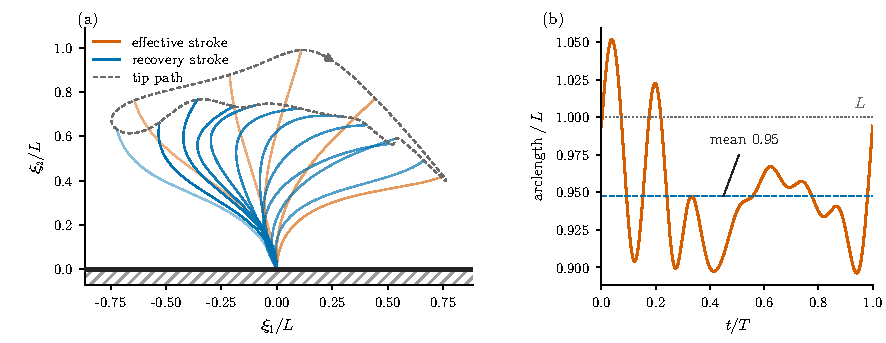
\includegraphics[width=\textwidth]{beat.pdf}
  \caption{The Fulford--Blake beat. (a) Centreline shapes at 16 equally spaced phases of one cycle, coloured by stroke, and the path of the tip. (b) Arclength of the centreline over the cycle. The fit is not inextensible: the length changes by about 15\,\% over the beat, which is why panel lengths are taken from the true arclength (Sec.~\ref{sec:panels}).}
  \label{fig:beat}
\end{figure}

\subsection{Panels}
\label{sec:panels}
Each cilium is cut into $N_p$ panels centred at $s_i = (i-\tfrac12)/N_p$.
Because the Fulford--Blake fit does not keep $|\partial_s\vect X|$ fixed (Fig.~\ref{fig:beat}b), equal steps in $s$ are not equal lengths along the cilium.
The code therefore gives panel $i$ its true arclength and the analytic unit tangent,
\begin{equation}
  l_i = \frac{L_c}{N_p}\,\bigl|\partial_s \vect\xi(s_i,t)\bigr|,
  \qquad
  \vect t_i = \frac{\partial_s\vect X_k(s_i,t)}{|\partial_s\vect X_k(s_i,t)|},
\end{equation}
so that the sum over panels is the midpoint rule for the drag integrated along the actual curve (\code{panelLength = arclength}).
Using uniform lengths $L_c/N_p$ instead integrates over the parameter $s$ and lowers the mean pumping by about 5\,\%.

\section{Drag on each panel}

\begin{figure}[t]
  \centering
  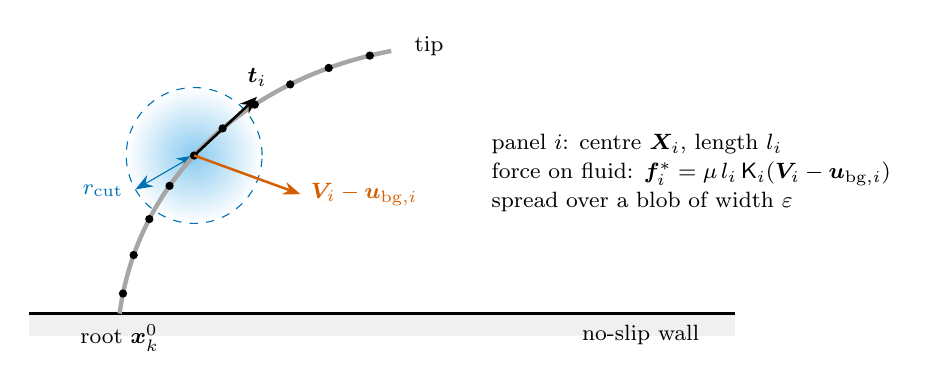
\begin{tikzpicture}[scale=1.15, >={Stealth[length=2.2mm]}]
    % wall
    \fill[gray!12] (-0.4,-0.25) rectangle (7.4,0);
    \draw[line width=1pt] (-0.4,0) -- (7.4,0);
    \node[anchor=north west, font=\footnotesize] at (5.6,-0.02) {no-slip wall};
    % blob around panel 5 (drawn first so the cilium sits on top)
    \coordinate (P) at (1.423,1.746);
    \shade[inner color=oisky!70, outer color=white] (P) circle (0.75);
    \draw[dashed, oiblue] (P) circle (0.75);
    \draw[<->, oiblue, thin] (P) -- ++(-150:0.75);
    \node[oiblue, font=\footnotesize, anchor=east] at ($(P)+(-150:0.78)$) {$r_\mathrm{cut}$};
    % cilium centreline with panel centres at s_i = (i - 1/2)/N_p
    \draw[line width=1.6pt, gray!70] (0.6,0) .. controls (0.8,1.5) and (2.0,2.6) .. (3.6,2.9)
      \foreach \q in {0.05,0.15,0.25,0.35,0.45,0.55,0.65,0.75,0.85,0.95} {node[pos=\q, circle, fill=black, inner sep=0pt, minimum size=3pt] {}};
    % tangent and relative velocity at panel 5
    \draw[->, line width=0.9pt, black] (P) -- ++(43:0.95) node[above, font=\footnotesize] {$\vect t_i$};
    \draw[->, line width=0.9pt, oiverm] (P) -- ++(-20:1.25) node[right, font=\footnotesize] {$\vect V_i - \vect u_{\mathrm{bg},i}$};
    \node[font=\footnotesize, anchor=west] at (3.75,2.95) {tip};
    \node[font=\footnotesize, anchor=north] at (0.6,-0.02) {root $\vect x_k^0$};
    % legend text
    \node[align=left, font=\footnotesize, anchor=west] at (4.6,1.55) {%
      panel $i$: centre $\vect X_i$, length $l_i$\\[1pt]
      force on fluid: $\vect f^*_i = \mu\, l_i\, \tens K_i(\vect V_i - \vect u_{\mathrm{bg},i})$\\[1pt]
      spread over a blob of width $\eps$};
  \end{tikzpicture}
  \caption{One actuator filament. Each panel (dots) samples the background velocity $\vect u_\mathrm{bg}$ at its centre, turns the slip into a force with the anisotropic resistance $\tens K_i$ of resistive-force theory, and returns that force to the fluid as a regularised body force of width $\eps$, truncated at $r_\mathrm{cut}$ (shaded).}
  \label{fig:schematic}
\end{figure}

The force that panel $i$ exerts on the fluid is the resistive-force-theory drag of a slender filament~\cite{GrayHancock1955,Lighthill1976},
\begin{equation}
  \vect f^{*}_i = R(t)\,\mu\, l_i\,\tens K_i\,\bigl(\vect V_i - \vect u_{\mathrm{bg},i}\bigr),
  \qquad
  \tens K_i = C_\parallel\,\vect t_i\vect t_i^{\mathsf T} + C_\perp\bigl(\tens I - \vect t_i\vect t_i^{\mathsf T}\bigr),
  \label{eq:rft}
\end{equation}
\begin{equation}
  C_\parallel = \frac{2\pi}{\ln(L/r)}, \qquad C_\perp = 2\,C_\parallel ,
\end{equation}
where $r$ is the cilium radius ($L/r = 20$) and $R(t) = \min(1, t/T_\mathrm{ramp})$ ramps the force up over the first $T_\mathrm{ramp} = 0.01$ to avoid an impulsive start.
The panel is pulled along by the prescribed motion, so $\vect f^*_i$ points along the slip $\vect V_i - \vect u_{\mathrm{bg},i}$, twice as strongly across the filament as along it (Fig.~\ref{fig:schematic}).
The fluid velocity at the panel centres is found with nekRS's spectral point interpolation; panels are first wrapped into the periodic box.

\subsection{Removing the filament's own flow}

The coefficients $C_\parallel$ and $C_\perp$ already contain the flow a slender filament induces along itself: that is where the $\ln(L/r)$ comes from.
The velocity $\vect u(\vect X_i)$ read off the grid also contains it, because the cilium's own spread force drives flow at its panels.
Using $\vect u$ in \eqref{eq:rft} counts the self-flow twice and delivers only about half of the intended drag (52\,\% across and 61\,\% along a straight rod at $\eps = 0.1$; Sec.~\ref{sec:verification}), and the shortfall grows as $\eps$ shrinks.
The same effect is known for actuator-line models of turbine blades, where it is removed by the filtered lifting-line correction~\cite{MartinezTossasMeneveau2019}.
The Stokes counterpart used here (\code{subtractSelfFlow = 1}) subtracts the free-space regularised Stokeslet flow of the cilium's own panels,
\begin{equation}
  \vect u_{\mathrm{bg},i} = \vect u(\vect X_i) - \frac{1}{\mu}\sum_{j\,\in\,\text{cilium }k} \tens S_\eps(\vect X_i - \vect X_j)\,\vect F_j ,
  \label{eq:selfflow}
\end{equation}
where $\vect F_j$ is the force that produced $\vect u$ and $\tens S_\eps$ is the Stokeslet regularised by the spreading kernel of Sec.~\ref{sec:spreading}~\cite{Cortez2001,CortezFauciMedovikov2005}.
For the Gaussian blob, with $\rho = r/\eps$,
\begin{gather}
  \tens S_\eps(\vect r) = a(r)\,\tens I + b(r)\,\hat{\vect r}\hat{\vect r}^{\mathsf T},
  \qquad a = G - \frac{B'}{r}, \qquad b = \frac{3B'}{r} - G, \\
  G = \frac{\operatorname{erf}\rho}{4\pi r},
  \qquad
  B' = \frac{1}{4\pi r^2}\Bigl[\Bigl(\frac{r^2}{2} - \frac{\eps^2}{4}\Bigr)\operatorname{erf}\rho + \frac{\eps r}{2\sqrt\pi}\,e^{-\rho^2}\Bigr],
\end{gather}
and for the zero-second-moment blob $G \to G + \tfrac{\eps^2}{4}\,\delta^{\mathrm{G}}_\eps$, $B' \to B' - \tfrac{\eps^2}{4}\,G'$.
Only the cilium's own free-space flow is removed: the wall, the periodic images and the other cilia are not in resistive-force theory and stay in $\vect u_\mathrm{bg}$.

\section{Spreading the forces onto the grid}
\label{sec:spreading}

The panel forces enter \eqref{eq:stokes} as
\begin{equation}
  \vect f_b(\vect x) = \sum_{k}\sum_{i=1}^{N_p} \vect F_{k,i}\;\delta_\eps\bigl(\vect x - \vect X_{k,i}\bigr),
\end{equation}
with distances taken by the minimum-image rule in $x$ and $y$.
The default kernel (\code{gaussianKernel = gauss2}) is the Gaussian corrected to have zero second moment,
\begin{equation}
  \delta^{\mathrm{G}}_\eps(r) = \frac{e^{-r^2/\eps^2}}{\pi^{3/2}\eps^3},
  \qquad
  \delta_\eps(r) = \Bigl(\frac52 - \frac{r^2}{\eps^2}\Bigr)\,\delta^{\mathrm{G}}_\eps(r)
  = \Bigl(1 - \frac{\eps^2}{4}\nabla^2\Bigr)\delta^{\mathrm{G}}_\eps .
  \label{eq:kernel}
\end{equation}
Both kernels carry unit force.
The plain Gaussian $\delta^\mathrm{G}_\eps$ has a second moment, so the flow it drives differs from a point Stokeslet by a potential dipole of strength $O(\eps^2)$, an $O(\eps^2/d^3)$ error in every interaction at distance $d$: with the wall image of the cilium itself and with its neighbours.
The correction in \eqref{eq:kernel} cancels that term, so beyond a few $\eps$ the flow of $\delta_\eps$ is the point Stokeslet up to exponentially small terms.
The kernel is truncated at $r_\mathrm{cut} = 3.8\,\eps$, beyond which it carries $3\times10^{-5}$ of the force (Fig.~\ref{fig:kernels}).

In this model $\eps$ is a numerical width, not the cilium radius: the radius is already in $C_\parallel$ and $C_\perp$, and once the self-flow is removed the answer converges as $\eps\to0$ at fixed $\eps/\Delta x$ and $\eps/(L/N_p)$.
The default $\eps = 0.1$ with $N_p = 40$ is resolved on the benchmark mesh: against $N_p = 80$, the mean wall shear differs by 0.38\,\% (1.9\,\% at $N_p = 20$), at about second order in $N_p$.

\begin{figure}[t]
  \centering
  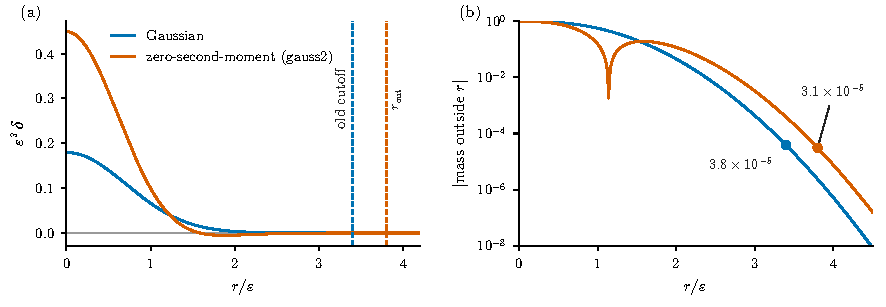
\includegraphics[width=\textwidth]{kernels.pdf}
  \caption{Spreading kernels. (a) Radial profiles of the Gaussian and of the zero-second-moment kernel \eqref{eq:kernel}; dashed lines mark the truncation radii. (b) Magnitude of the force carried outside radius $r$; for the zero-second-moment kernel it changes sign near $r = 1.1\,\eps$ (the cusp), and the labels give the values at the truncation radii.}
  \label{fig:kernels}
\end{figure}

The spreading is one OCCA kernel, \code{addCiliaForce}, run on the device: every quadrature point loops over the panels and adds those within $r_\mathrm{cut}$, rejecting one coordinate at a time.
Its result, multiplied by the mass matrix, is added straight into the assembled right-hand side of the step, so the cilia force is evaluated at $t_{n+1}$ and never extrapolated.

\section{Coupling forces and flow}

Equations \eqref{eq:rft}--\eqref{eq:selfflow} close the model only if the force applied to the fluid is the drag computed from the flow it produces, $\vect F = \vect f^*$.
Within a time step define $H(\vect F)$: apply the panel forces $\vect F$ at $\vect X(t_{n+1})$, solve \eqref{eq:stokes} for $\vect u^{n+1}$, and return $\vect f^*$ from \eqref{eq:rft}.
The model is the fixed point
\begin{equation}
  \vect F^{n+1} = H(\vect F^{n+1}).
  \label{eq:fixedpoint}
\end{equation}
An explicit scheme that uses the forces from $\vect u^n$ is unstable for this model: the loop gain from force to sampled velocity and back is close to one, and a filter that damps it (relaxing $\vect f$ towards $\vect f^*$ with a cut-off frequency $f_c$) changes the answer, by about $-35\,\%$ in mean pumping at $f_c = 1.59f$.
The code therefore solves \eqref{eq:fixedpoint} with outer correctors and interface quasi-Newton least squares (IQN-ILS)~\cite{Degroote2009}, the scheme used in partitioned fluid--structure interaction (Fig.~\ref{fig:loop}):
\begin{enumerate}
  \item \emph{Predictor.} $\vect F^{(1)} = \sum_h c^\mathrm{EXT}_h\,\vect F^{n-h}$, the converged forces of the last steps extrapolated with the solver's own EXT coefficients.
  \item \emph{Corrector $k$.} Spread $\vect F^{(k)}$, solve, sample $\vect u$, subtract the self-flow of $\vect F^{(k)}$, and form $\vect H^{(k)} = H(\vect F^{(k)})$ and the residual $\vect r^{(k)} = \vect H^{(k)} - \vect F^{(k)}$.
  \item \emph{Stop} when $\|\vect r^{(k)}\| \le \tau\,\|\vect H^{(k)}\|$, with $\tau = 3\times10^{-5}$ (2-norm over all panels).
  \item \emph{Update.} With the secant differences $\Delta\vect r$ and $\Delta\vect H$ of this step and of the last $q = 8$ steps as columns of $\tens V$ and $\tens W$, solve $\vect c = \arg\min\|\tens V\vect c + \vect r^{(k)}\|$ by QR (dropping nearly dependent columns) and set $\vect F^{(k+1)} = \vect H^{(k)} + \tens W\vect c$. Without any secant pairs, $\vect F^{(k+1)} = \vect F^{(k)} + 0.2\,\vect r^{(k)}$.
\end{enumerate}
In Stokes flow $H$ is affine in $\vect F$ within a step, so the secant model is close to exact; the benchmark needs 2.3 fluid solves per step on average.
The correctors are run by nekRS's own outer-iteration hook (\code{userConvergenceCheck}), so each one is a normal pressure and velocity solve.

\begin{figure}[t]
  \centering
  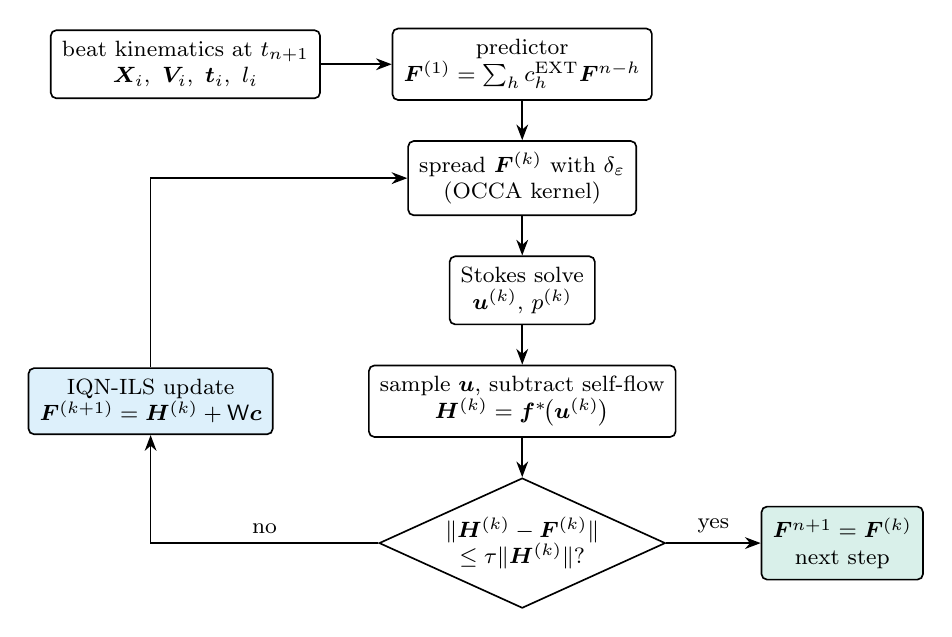
\begin{tikzpicture}[
      node distance=5mm and 9mm,
      box/.style={draw, rounded corners=2pt, align=center, font=\footnotesize, minimum height=8mm, inner sep=4pt, fill=white},
      dec/.style={draw, diamond, aspect=2.2, align=center, font=\footnotesize, inner sep=1pt, fill=white},
      >={Stealth[length=2mm]}, line width=0.6pt]
    \node[box] (kin) {beat kinematics at $t_{n+1}$\\ $\vect X_i,\ \vect V_i,\ \vect t_i,\ l_i$};
    \node[box, right=of kin] (pred) {predictor\\ $\vect F^{(1)} = \sum_h c^\mathrm{EXT}_h \vect F^{n-h}$};
    \node[box, below=of pred] (spread) {spread $\vect F^{(k)}$ with $\delta_\eps$\\ (OCCA kernel)};
    \node[box, below=of spread] (solve) {Stokes solve\\ $\vect u^{(k)}$, $p^{(k)}$};
    \node[box, below=of solve] (rft) {sample $\vect u$, subtract self-flow\\ $\vect H^{(k)} = \vect f^*\!\bigl(\vect u^{(k)}\bigr)$};
    \node[dec, below=of rft] (conv) {$\|\vect H^{(k)} - \vect F^{(k)}\|$\\ $\le \tau\|\vect H^{(k)}\|$?};
    \node[box, left=12mm of rft, fill=oisky!20] (iqn) {IQN-ILS update\\ $\vect F^{(k+1)} = \vect H^{(k)} + \tens W\vect c$};
    \node[box, right=12mm of conv, fill=oigreen!15] (next) {$\vect F^{n+1} = \vect F^{(k)}$\\ next step};
    \draw[->] (kin) -- (pred);
    \draw[->] (pred) -- (spread);
    \draw[->] (spread) -- (solve);
    \draw[->] (solve) -- (rft);
    \draw[->] (rft) -- (conv);
    \draw[->] (conv) -- node[above, font=\footnotesize] {yes} (next);
    \draw[->] (conv.west) -| node[pos=0.25, above, font=\footnotesize] {no} (iqn.south);
    \draw[->] (iqn.north) |- (spread.west);
  \end{tikzpicture}
  \caption{One time step. Outer correctors repeat the fluid solve with updated panel forces until the applied force equals the drag it produces; IQN-ILS builds the update from the secant history of this and earlier steps.}
  \label{fig:loop}
\end{figure}

\paragraph{Time integration.}
nekRS advances \eqref{eq:stokes} with second-order backward differences (BDF2) at $\Delta t = 10^{-3}T$, i.e.\ 1000 steps per beat, with residual tolerances $3\times10^{-3}$ for pressure and velocity.
The beat is prescribed analytically, so the only coupling error is the residual tolerance $\tau$.

\section{Diagnostics}
Every step the udf prints two lines that the regression gate (\code{gate.py}) reads: the volume-mean velocity $\bar u$ and $\max|\vect u|$, and the integrals of $u$, $p$, $\partial u/\partial z$ and $\partial v/\partial z$ over the horizontal plane $z = 0.001$ and over the wall.
The plane integrals use the element quadrature with the Lagrange interpolant in $z$, so they are exact for the spectral solution, and run as one fused device reduction.
On the wall, $\mu\int\partial u/\partial z$ and $\mu\int\partial v/\partial z$ are the total shear force the cilia exert on the epithelium.

\section{Benchmark case and parameters}

\begin{figure}[t]
  \centering
  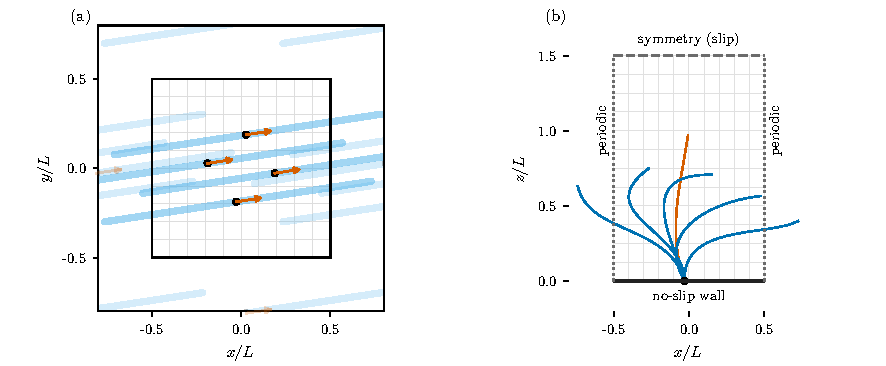
\includegraphics[width=\textwidth]{layout.pdf}
  \caption{The \code{small4} benchmark. (a) Top view: four roots on a square lattice, all beating in the cell direction (arrows), with the footprint of each beat plane and the neighbouring periodic copies (faint). (b) Side view with the spectral-element grid ($10\times10\times12$ elements, polynomial order 5) and one cilium through the cycle.}
  \label{fig:layout}
\end{figure}

\code{cases/small4} is four cilia in a $1\times1\times1.5$ box (Fig.~\ref{fig:layout}).
The roots form a $2\times2$ patch with spacing $0.269$, taken from one basal-body patch of a ciliated cell (hexagonal cells of side $5\,\mu$m, cilia $6\,\mu$m long).
Every cilium in a cell beats in the cell's direction ($\beta_k = \alpha$, $\alpha$ drawn from $\mathcal N(0, 25^\circ)$), in phase, and the root lattice is turned $28^\circ$ from the beat so that neighbours stay at least $0.126\,L > 2r$ apart over the whole cycle.
The periodic box makes this a patch of an infinite carpet; the kernels of neighbouring cilia overlap, as they do in dense ciliated tissue.
Table~\ref{tab:params} lists the defaults, all set in the \code{[CASEDATA]} section of \code{small4.par}.

\begin{table}[h]
  \centering
  \small
  \caption{Model parameters of \code{small4} (units of $L$ and $T$).}
  \label{tab:params}
  \begin{tabular}{@{}llll@{}}
    \toprule
    Quantity & Symbol & Value & \code{[CASEDATA]} key \\
    \midrule
    Reynolds number & $\mathrm{Re}$ & $10^{-3}$ & (\code{[FLUID VELOCITY] viscosity}) \\
    Panels per cilium & $N_p$ & 40 & \code{numPanels} \\
    Slenderness & $L/r$ & 20 & \code{slenderness} \\
    Kernel & $\delta_\eps$ & zero second moment & \code{gaussianKernel = gauss2} \\
    Kernel width & $\eps$ & 0.1 & \code{gaussianWidth} \\
    Kernel truncation & $r_\mathrm{cut}/\eps$ & 3.8 & \code{gaussianCutoff} \\
    Panel lengths & $l_i$ & true arclength & \code{panelLength = arclength} \\
    Self-flow removal & & on & \code{subtractSelfFlow = 1} \\
    Coupling & & IQN-ILS, $q = 8$ & \code{couplingScheme = iqn} \\
    Coupling tolerance & $\tau$ & $3\times10^{-5}$ & \code{couplingTol} \\
    Start-up ramp & $T_\mathrm{ramp}$ & 0.01 & \code{rampTime} \\
    Time step & $\Delta t$ & $10^{-3}$ & (\code{[GENERAL] dt}) \\
    Polynomial order & $N$ & 5 & (\code{[GENERAL] polynomialOrder}) \\
    \bottomrule
  \end{tabular}
\end{table}

\section{Verification}
\label{sec:verification}

\paragraph{Straight rod.}
A rigid straight rod ($L = 1$, $N_p = 20$) held at the centre of a cubic box of side $B$ with a virtual velocity of 1 should feel the resistive-force-theory drag.
Runs at $B = 4$ and $8$, extrapolated linearly in $1/B$ to free space, give:
\begin{center}
  \small
  \begin{tabular}{@{}lccc@{}}
    \toprule
    Drag / RFT, $B\to\infty$ & raw $\vect u$ & with \eqref{eq:selfflow} & free-space estimate, raw \\
    \midrule
    across the rod ($\eps = 0.1$) & 0.518 & 0.983 & 0.520 \\
    along the rod ($\eps = 0.1$)  & 0.613 & 0.996 & 0.614 \\
    \bottomrule
  \end{tabular}
\end{center}
With the self-flow removed, the drag at $B = 4$ is the same for $\eps = 0.1$ and $0.05$ to $10^{-4}$; without it, halving $\eps$ loses another 12\,\%.

\paragraph{Regression gate.}
\code{gate.py} compares the second beat cycle of a \code{small4} run with a reference computed at $\Delta t = 10^{-4}$, $\tau = 10^{-5}$ and solver tolerances $10^{-4}$.
A quantity passes if its largest deviation over the cycle is at most $0.1\,\%$ of its peak; the production settings pass with $8.7\times10^{-4}$ on the worst quantity ($\int\partial v/\partial z$).

\begin{thebibliography}{9}\small
\bibitem{FulfordBlake1986}
G.~R. Fulford and J.~R. Blake, Muco-ciliary transport in the lung, \emph{J.\ Theor.\ Biol.}\ \textbf{121}, 381--402 (1986).
\bibitem{GrayHancock1955}
J.~Gray and G.~J. Hancock, The propulsion of sea-urchin spermatozoa, \emph{J.\ Exp.\ Biol.}\ \textbf{32}, 802--814 (1955).
\bibitem{Lighthill1976}
J.~Lighthill, Flagellar hydrodynamics, \emph{SIAM Rev.}\ \textbf{18}, 161--230 (1976).
\bibitem{Cortez2001}
R.~Cortez, The method of regularized Stokeslets, \emph{SIAM J.\ Sci.\ Comput.}\ \textbf{23}, 1204--1225 (2001).
\bibitem{CortezFauciMedovikov2005}
R.~Cortez, L.~Fauci and A.~Medovikov, The method of regularized Stokeslets in three dimensions: analysis, validation, and application to helical swimming, \emph{Phys.\ Fluids} \textbf{17}, 031504 (2005).
\bibitem{MartinezTossasMeneveau2019}
L.~A. Mart\'inez-Tossas and C.~Meneveau, Filtered lifting line theory and application to the actuator line model, \emph{J.\ Fluid Mech.}\ \textbf{863}, 269--292 (2019).
\bibitem{Degroote2009}
J.~Degroote, K.-J. Bathe and J.~Vierendeels, Performance of a new partitioned procedure versus a monolithic procedure in fluid--structure interaction, \emph{Comput.\ Struct.}\ \textbf{87}, 793--801 (2009).
\bibitem{nekRS}
P.~Fischer \emph{et al.}, NekRS, a GPU-accelerated spectral element Navier--Stokes solver, \emph{Parallel Comput.}\ \textbf{114}, 102982 (2022).
\end{thebibliography}

\end{document}
